\documentclass[11pt,a4paper,oldfontcommands]{memoir}
\usepackage[utf8]{inputenc}
\usepackage[T1]{fontenc}
\usepackage{microtype}
\usepackage[dvips]{graphicx}
\usepackage{xcolor}
\usepackage{times}
\usepackage{amsmath}

\usepackage[
breaklinks=true,colorlinks=true,
%linkcolor=blue,urlcolor=blue,citecolor=blue,% PDF VIEW
linkcolor=black,urlcolor=black,citecolor=black,% PRINT
bookmarks=true,bookmarksopenlevel=2]{hyperref}

\usepackage{geometry}
% PDF VIEW
% \geometry{total={210mm,297mm},
% left=25mm,right=25mm,%
% bindingoffset=0mm, top=25mm,bottom=25mm}
% PRINT
\geometry{total={210mm,297mm},
left=20mm,right=20mm,
bindingoffset=10mm, top=25mm,bottom=25mm}

\OnehalfSpacing
%\linespread{1.3}

%%% CHAPTER'S STYLE
\chapterstyle{bianchi}
%\chapterstyle{ger}
%\chapterstyle{madsen}
%\chapterstyle{ell}
%%% STYLE OF SECTIONS, SUBSECTIONS, AND SUBSUBSECTIONS
\setsecheadstyle{\Large\bfseries\sffamily\raggedright}
\setsubsecheadstyle{\large\bfseries\sffamily\raggedright}
\setsubsubsecheadstyle{\bfseries\sffamily\raggedright}


%%% STYLE OF PAGES NUMBERING
%\pagestyle{companion}\nouppercaseheads 
%\pagestyle{headings}
%\pagestyle{Ruled}
\pagestyle{plain}
\makepagestyle{plain}
\makeevenfoot{plain}{\thepage}{}{}
\makeoddfoot{plain}{}{}{\thepage}
\makeevenhead{plain}{}{}{}
\makeoddhead{plain}{}{}{}


\maxsecnumdepth{subsection} % chapters, sections, and subsections are numbered
\maxtocdepth{subsection} % chapters, sections, and subsections are in the Table of Contents


%%%---%%%---%%%---%%%---%%%---%%%---%%%---%%%---%%%---%%%---%%%---%%%---%%%

\begin{document}

%%%---%%%---%%%---%%%---%%%---%%%---%%%---%%%---%%%---%%%---%%%---%%%---%%%
%   TITLEPAGE
%
%   due to variety of titlepage schemes it is probably better to make titlepage manually
%
%%%---%%%---%%%---%%%---%%%---%%%---%%%---%%%---%%%---%%%---%%%---%%%---%%%
\thispagestyle{empty}

{%%%
\sffamily
\centering
\Large

~\vspace{\fill}

{\huge 
Finite Element Analysis in Time Domain and Eigenspace
}

\vspace{2.5cm}

{\LARGE
Darwin Li
}


\vspace{\fill}

December 2016

%%%
}%%%

\cleardoublepage
%%%---%%%---%%%---%%%---%%%---%%%---%%%---%%%---%%%---%%%---%%%---%%%---%%%
%%%---%%%---%%%---%%%---%%%---%%%---%%%---%%%---%%%---%%%---%%%---%%%---%%%

\tableofcontents*

\clearpage

%%%---%%%---%%%---%%%---%%%---%%%---%%%---%%%---%%%---%%%---%%%---%%%---%%%
%%%---%%%---%%%---%%%---%%%---%%%---%%%---%%%---%%%---%%%---%%%---%%%---%%%

\chapter{Introduction}

\section{Motivation}
Of the full wave numerical methods for electromagnetics on the market, one of the least available is the Finite Element Time domain algorithm. The greater goal of this project is to create an open-source code that can read in arbitrary meshes generated by open-source mesh engines and use open-source matrix libraries such as Apache Math Commons~\cite{ApacheMathCommon} to generate a time-domain solution. This would be very powerful since a Tetrahedral mesh can conform to structures, and a time-domain solution inherently gives more information than a frequency-domain solution. Due to the complexity of Finite Element Analysis in three dimensions with vectors, I chose Java as the language because of the many data structures that are readily available to make the Book keeping as straightforward as possible.

The short term goal of this project aims to take in any 3D cavity structure (though it has only been tested for Rectangular) produced by gmsh and output some important Electromagnetic properties. For an arbitrary Cavity, all boundaries can be treated as Electrically conducting, so the associated property would be the eigenvalues (wave numbers) sustained in such a cavity. Another specific case is if we take a very thin (short in the z-direction) rectangular cavity and treat the Zmax and Zmin as electrically conducting, but the other 4 walls as magnetically conducting. This treatment is important for Power Delivery Network analysis where we can ignore the fringing electric fields at the end of the plane ~\cite{Swaminathan}.

The former experiment is an eigenmode problem by nature, and can be done using the Finite Element Method (FEM) simply by solving the eigenvalues of matrices to get a limited range of resonant frequencies. The latter experiment requires a much broader range of frequencies, and so it is more efficient to use a Finite Element in Time domain (FETD) algorithm. One can think of the FETD algorithm as an extension to the FEM algorithm, but with an extra treatment for the time-stepping and source.

\section{Instructions to Run}
Upon running the .jar file, the user is prompted for the location of the .msh file, where to save the outputs, and which type of problem the user would like to solve. Currently for the dieletric constants, the user has to change it manually in the PhysicsConstants.java file.

A typical Eigenmode Analysis input would look like this, where the first 1.0 corresponds to the minimum Frequency in Hz. The choice of Eigenmode problem is given by the first non decimaled 1.

C:\textbackslash Users\textbackslash darwinli\textbackslash Documents\textbackslash projMesh \textbackslash box.msh
\\ C:\textbackslash Users\textbackslash darwinli\textbackslash Documents\textbackslash ProjectFiles
\\ 0.0
\\ 10.0
\\ 1
\\ 1


For the case of FETD, more user input is required for the frequency range, the location of the current source which can be determined from~\cite{Swaminathan}, and the location of the voltage monitor (to monitor the time domain waveform at another location in the domain).


A typical FETD input would look like this:

C:\textbackslash Users\textbackslash darwinli\textbackslash Documents\textbackslash projMesh\textbackslash  planes.msh
\\C:\textbackslash Users\textbackslash darwinli\textbackslash Documents\textbackslash ProjectFiles
\\1e6
\\1e9
\\2
\\0.0625,0.05
\\0.0725,0.06
\\100




\chapter{Coding}

\section{Electromagnetics Derivations}

\subsection{Weak Formulation of the Boundary Value Problem}
Finite Element Analysis for Computational Electromagnetics starts with the boundary-value problem:
\begin{equation} \label{eq:1}
L\phi = f
\end{equation}

With L as a differential operator, and f as the forcing function, the goal is to solve phi. At this point there are multiple methods to choose from to approximate the solution such as the Rayleigh-Ritz method ~\cite{Jin2}, but I will use Gelarkin’s method of weighted residuals. This means that we can break the domain up into N parts, treating the equation 1 as an integration over all parts so that we can solve the problem as 

\begin{equation} \label{eq:2}
\sum_{j=0}^{N}c_j\int_{\Omega}v_iL(v_j) d\Omega
\end{equation}

A weak formulation must now  be created with the principles of electromagnetics . The full derivation can be found in ~\cite{Jin}, but the final equation is shown below after taking Helmholtz's equation based only on the E-Field:

\begin{equation} \label{eq:3}
\nabla\times (\frac{1}{\mu_r}\nabla \times \mathbf{E}) - k_{0}^{2}\epsilon_{r}\mathbf{E} = -jk_{0}Z_{0}\mathbf{J} \textrm{ on } \Omega
\end{equation}

The suitable weak-form being:

$\int_{\Omega}[(\nabla\times \mathbf{W_i}) \cdot (\frac{1}{\mu_r}\nabla \times \mathbf{E}) - k_{0}^{2}\epsilon_{r}\mathbf{W_i}\cdot\mathbf{E}]d\Omega = \int_{\Gamma_{D}} \frac{1}{\mu_r}(\hat{n}\times \mathbf{W_i})\cdot(\nabla \times \mathbf{E})d\Gamma$ 

$-  \int_{\Gamma_{N}}[\frac{jk_0}{\eta}(\hat{n} \times \mathbf{W_i})\cdot(\hat{n}\times\mathbf{E}) + \mathbf{W_i} \cdot \mathbf{K}_N] d\Gamma - jk_0 Z_0 \int_{\Omega}\mathbf{W_i}\cdot \mathbf{J} d\Omega$


Where $\mathbf{W_i}$ is our weighting function.

For a full-wave 3D solver, it works best if we try to solve for the Electric Field directly at an edge rather than solving for the voltage at a node. This is stated in many texts ~\cite{Jin}.  So, if we treat our linear interpolating functions as maximum when they are on their respective edge, we find that the basis function E-Fields are defined tangentially along each edge.  

For the two terms in the left integral, we can split them into two separate integrals and treat them as a set of matrices with elements defined as such now with $\mathbf{N_i}$ defined as our interpolating function which through Gelarkin's method can replace $\mathbf{W_i}$ and $\mathbf{E_i}$. 

\begin{equation} \label{eq:4}
S_{ij} = \int \int \int_{S} \nabla\times\mathbf{N_i} \cdot \nabla\times\mathbf{N_j} dS
\end{equation}

\begin{equation} \label{eq:5}
T_{ij} = \int \int \int_{S} \mathbf{N_i} \cdot \mathbf{N_j} dS
\end{equation}

Notice that the constants are cleansed from these equations since the constants will be treated differently for the FEM case and for the FETD case. Although we are using a edge-based interpolating function, it is still not possible to remove the necessity to compute based on the nodes in our domain. This is simply because a finite edge in 3 dimensions is identified by 2 nodes, so without explicitly processing the information of each node, it is impossible for this treatment to work. As such, we define the interpolating function $\mathbf{N}$ for the edge as:

\begin{equation} \label{eq:6}
\mathbf{N_i} = \lambda_{i1} \nabla \lambda_{i2} - \lambda_{i2} \nabla \lambda_{i1}
\end{equation}

The numbering scheme for each $\lambda$ now must have 2 indices, with the first one being the edge element it is being treated on, and the second being the ordered pair index on the edge element. Each edge element is a vector and points from Node 1 to Node 2, hence the second index is always either 1 or 2. We can define the $\lambda$, our linear poly(1) interpolation as follows:

\begin{equation} \label{eq:7}
\lambda_{i} = a_i + b_i x + c_i y + d_i z
\end{equation}

To compute the constants, it can be shown through linear algebric maniuplation that:

$\begin{bmatrix}
       b_1 & c_1 & d_1 & a_1 \\ 
       b_2 & c_2 & d_2 & a_2 \\ 
       b_3 & c_3 & d_3 & a_3 \\ 
       b_4 & c_4 & d_4 & a_4 \\ 
\end{bmatrix}
= \begin{bmatrix}
       x_1 & x_2 & x_3 & x_4 \\ 
       y_1 & y_2 & y_3 & y_4 \\ 
       z_1 & z_2 & z_3 & z_4 \\ 
       1 & 1& 1 & 1 \\ 
\end{bmatrix}^{-1}$

By using the concept of local and global numbering system, we can treat each Element of 4 points as a local numbering system of 1 through 4 to do the computations and tie back to the global numbering system to do the summations to create the matrices.

\subsection{Java Classes}

The Element Class in my code represents a tetrahedron with 4 nodes. A Node is an object with an $x$, $y$, $z$ coordinate as well as a flag for whether it is on a Dirichilet boundary or not. It also has a flag for whether or not it lies on the current source or voltage monitor for the FETD case.

The Node flag for boundary is important because as shown by ~\cite{Jin}, the Dirichilet (PEC) condition requires explicit treatment for the boundary nodes. I will summarize quickly as follows since this treatment is generally accepted by all literature regarding Dirichilet Boundaries for Finite Element Analysis: By explicitly enforcing a constant value of 0 for the tangential E-Field, we are essentially forcing the basis functions of the edges lying on a boundary to be 0. As such, this places a constraint on all matrix terms that couple to the index of the edge lying on a boundary node. The easiest constraint is to make the column with the index of the dirichilet edge and row with the index of the Dirichilet edge equal to unity while the rest of the row in the matrix is 0. Then the rows and columns containing the index of the Dirichilet edge can be removed from all the matrices since for the PEC case, we want the value to be 0.

Though the MatrixCalcFETD and MatrixCalcEigenMode which extend Abstract Class MatrixCalc reads in the data, the actual computations are done in the Element objects themselves. For a consistent global system of edges, one requires a consistent local numbering scheme for each Node in an edge of an Element because edges are signed vectors. When computing the matrix components of $K_{ij}$, it is required that $K_{ij}^e$ be summed for all elements that have edges i and j, so it follows that if we are not consistent in treating the pair of nodes in an edge of an Element, then we will have a summation that is quite useless. 
The convention I have chosen is that each edge of an element MUST point from a globally lower numbered Node to a globally higher numbered Node where the global Node numbering is read in from the meshfile and kept in the Node object itself. So, the first step in instantiating an Element is that its array of Nodes be ordered from lowest global numbering to highest global numbering.
Then, care is placed when designating an edge locally with methods that explicitly take in or return a pair of nodes in the element. 
Of course, the global numbering scheme of the edges are important, so using our definition of an edge, it follows that an edge can be uniquely identified by its first Node and second Node. So, a HashMap is the most efficient datastructure to take in a pair of Nodes as a key and output an integer as the global edge number. Since keys cannot be duplicate, this data structure is the best for keeping track of our matrix indices.

Now, onto the Matrix construction.


\subsection{Matrix Construction}

The implementation of this computation is quite modular in my code. The computations are all done in the Element class itself to save time on iterating through each element. first I compute a private RealVector vVector(int e) which is just

\begin{equation} \label{eq:8}
\mathbf{v_{ij}} = \nabla\lambda_i \times \nabla\lambda_j
\end{equation}

Which through vector identities can be used to solve the $S$ matrix as such:

\begin{equation} \label{eq:9}
S_{ij} = 4\int\int\int_V \mathbf{v_{i1}} \cdot \mathbf{v_{i1}} dV
\end{equation}

Also note that $v_ij$ is independent of the  Simplex Coordinate Volume integrals since $\nabla\lambda$ has only constants
The Volume can also be calculated through the coordinates of a Tetrahedron. Please refer to the code for the treatment of Volume.

To compute the $T$ matrix, we define another helper function phi(int i, int j): $\phi_{ij} = \nabla \lambda_i \cdot \nabla \lambda_j$ where i and j are local node indeces.

Through vector identities, we can rewrite the $\mathbf{N_i}\cdot \mathbf{N_j}$ matrix elements in terms of $\phi$ and $\lambda$

\begin{equation} \label{eq:9}
\mathbf{N_i}\cdot \mathbf{N_j} = [\lambda_{i1}\lambda_{j1}(\nabla\lambda_{i2} \cdot \nabla\lambda_{j2}) - \lambda_{i2}\lambda_{j1}(\nabla\lambda_{i2}\cdot\nabla\lambda_{j1}) - \lambda_{i2}\lambda_{j1}(\nabla\lambda_{i1}\cdot\lambda_{j2}) + \lambda_{i2}\lambda_{j2}(\nabla\lambda_{i1} \cdot \nabla\lambda_{j1})]
\end{equation}

Also keeping in mind the simplex coordinate integral identity from ~\cite{Jin}


\begin{equation} \label{eq:9}
\int\int\int_{V} \lambda_{1}^{i}\lambda_{2}^{j}\lambda_{3}^{k}\lambda_{4}^{l} dV = \frac{3!i!j!k!l!}{(3+i+j+k+l)!}V
\end{equation}

It is important to note that we never have more than 2 lambda’s in one volume integra for these matricesl, and that the volume integral dissolves to either $2*V/20$ or $1*V/20$ corresponding respectively to if the two lambdas are on the exact same Node or on two different nodes.

Since the addMatrixTerms(HashMap<ArrayList<Integer>, Integer> iMap, HashMap<ArrayList<Integer>, Integer> dMap, RealMatrix r, 
    		RealMatrix t, RealMatrix s, RealVector f, HashSet<Integer> voltageSourceMonitor, 
    		HashSet<Integer> voltageMonitor1, HashSet<Integer> backwardsEdgeSet) function in Element takes in the Matrices themselves, then these matrix terms are added to the corresponding location in place such that when we finish iterating through all the elements, we have the full matrices.
This is an interesting method because at the same time as adding the Matrix terms, it also constructs the forcing vector (our source in FETD) and the monitors. The final parameter is a HashSet of backward edges so that when we take the integral of E-Field to get the Voltage, we are always integrating in one direction (since our sign of the E-Field along an edge is arbitrary with respect to any one of canonical axis).

For our forcing vector (which is applicable only to the FETD problem that requires a source):

\begin{equation} \label{eq:forcing}
f_i = \int\int\int_{V} \mathbf{N_i (r)}\cdot \frac{\partial \mathbf{J(r, t)}}{\partial t} dV
\end{equation}

We take the definition that the source Ji lies on the same edge as the interpolation function, so the dot product is simply their absolute values $N_i*\frac{\partial J}{\partial t}$, and we can compute the integral over $Ni$ with the formulation above. To compute $Ni$ we notice that it is just the square root of $\mathbf{Ni} \cdot \mathbf{Ni}$, so the integral of $f$ normalized to the current derivative is just the triple integral of $\sqrt{\mathbf{N_i} \cdot \mathbf{N_i}}$. This is no easy task, and must be done explicitly by taking the triple integral first for x, y, and then z. I make the assumption that this integral is approximately the one in {eq:11}. 

\chapter{Eigenmode Analysis of a Cavity}

The following analysis was originally done to check the matrix terms in anticipation of implementing FETD. Even though many tools on the market can compute this easily, it is still a non-trivial analysis, and the generality of it in an open-source project makes it important. Most of the following analysis is adopted from ~\cite{Davidson}

\section{Formulation of the problem}

The problem can be defined as 
\begin{equation} \label{eq:11}
F(\mathbf{E_t}) = [\frac{1}{2} \int\int_{S} \frac{1}{\mu_r} (\nabla \times \mathbf{E_t}) \cdot (\nabla \times \mathbf{E_t}) \cdot  - k_i^2 \epsilon_r \mathbf{E_t}\cdot\mathbf{E_t}] dS
\end{equation}

We set the above equation to 0 and notice that the first term in the integral is our $S$ Matrix and the second term is our $T$ Matrix. Thus, the eigen value problem is simply $[S] = k^2[T]$ where the wave numbers corresponding to the eigenmodes are the square root of the eigenvalues.

There is always the problem of the null vector space since the trivial solution is still a solution. Therefore, usually the first couple of Eigenvalues will be close to 0 and are not true Eigenvalues. Many resources point that this number is correlated to the number of free nodes in the system, but I have found that this is simply not true. For this reason, the user is required to input a fMin and fMax as the input before the start of the simulation so as to tell the system where the first real frequency should start.

\section{Results and validation}

For validation purposes, I will compare only to the fundamental mode, which is the TE mode for a long x dimension compared to y and z.The 1m x 0.5m x 0.75m box has the fundamental mode at 5.2359878 rad/m  
This was computed analytically from
\begin{equation} \label{eq:11}
k^{TE} = \sqrt{(\frac{n\pi}{a})^2 + \frac{m\pi}{b})^2 + \frac{l\pi}{c})^2}
\end{equation}

Mesh Refinement starts with the 10 nodes case and is refined through Splitting.
The initial mesh has 10 nodes and looks as such

\begin{figure}
  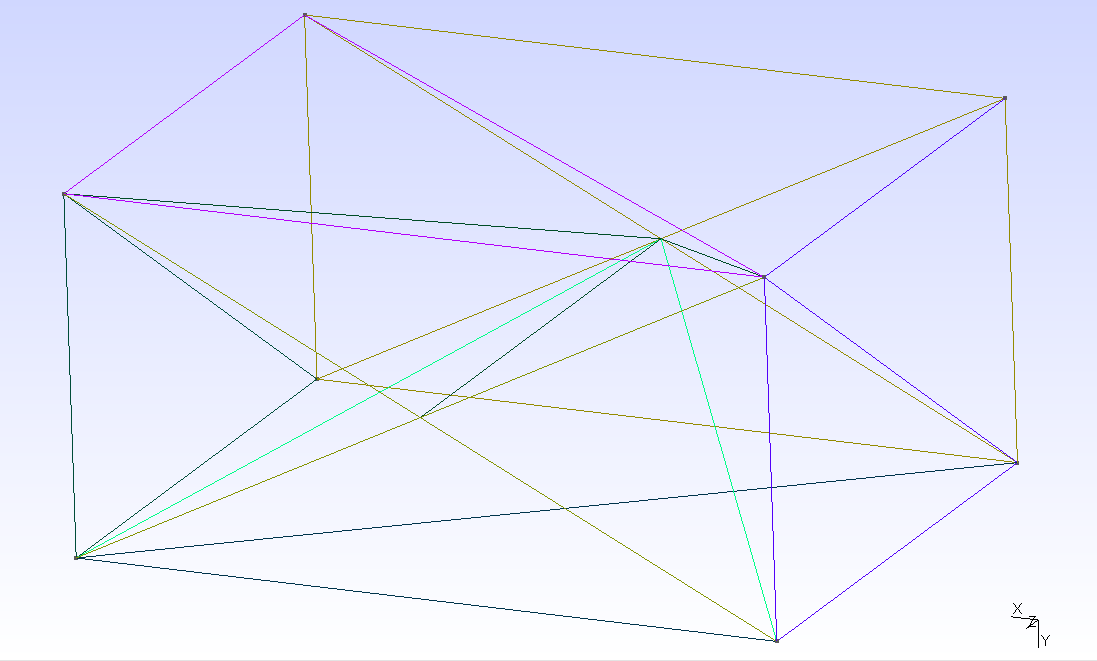
\includegraphics[width=\linewidth]{10Nodes.PNG}
  \caption{10 Nodes Mesh, no splits}
  \label{fig:mesh10}
\end{figure}

The value for 10 nodes is 5.498802 rad/m and this is a 0.2\%  error.
For 39 nodes the value is 5.379306 Rad/m with a 0.1\% error
For 205 nodes the vale is eigenvalue 5.264497 rad/m which is .03\% error.

\begin{figure}
  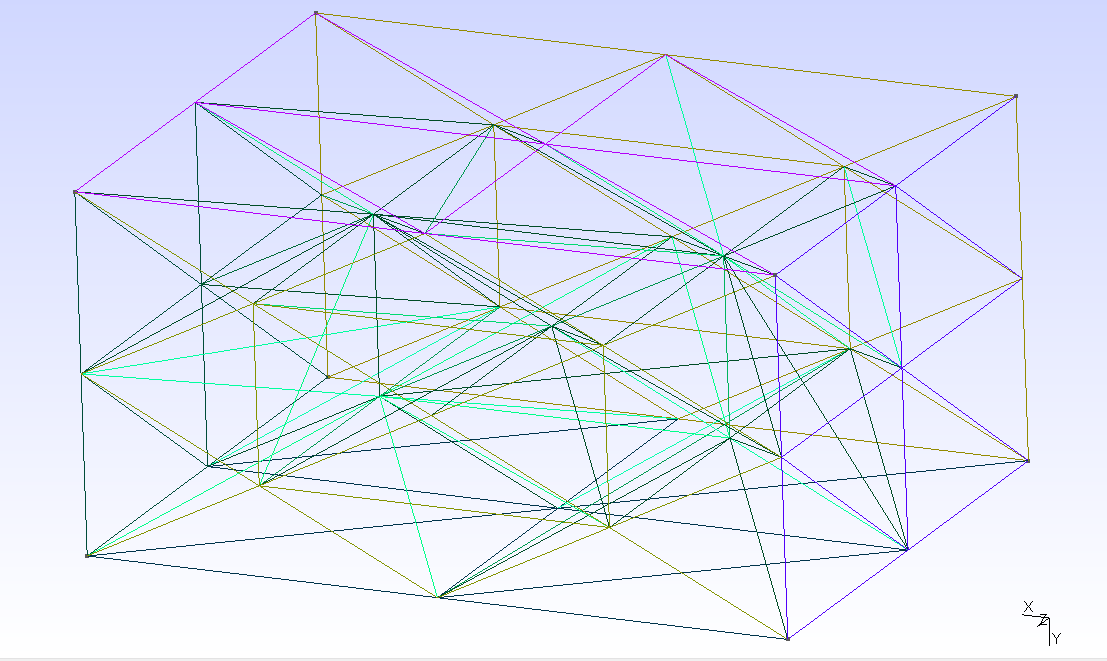
\includegraphics[width=\linewidth]{39Nodes.PNG}
  \caption{39 Nodes Mesh, First Split}
  \label{fig:mesh39}
\end{figure}

\begin{figure}
  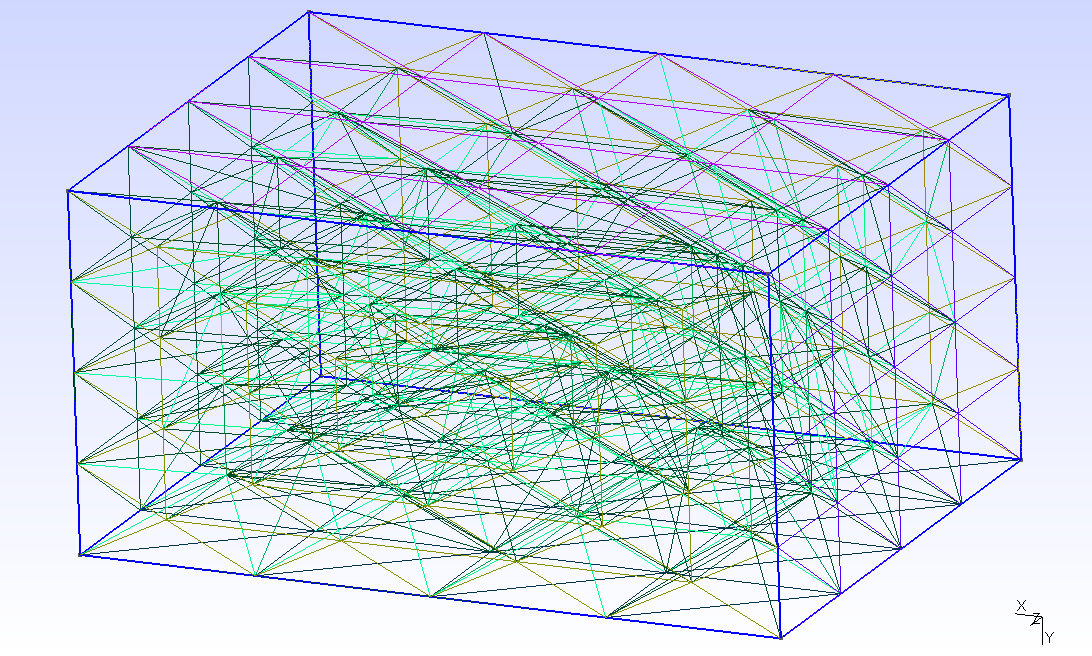
\includegraphics[width=\linewidth]{205Nodes.PNG}
  \caption{205Nodes Mesh, Second Split}
  \label{fig:mesh10}
\end{figure}


Overall this is a validation of the code. Performance-wise, Apache Commons Math ~\cite{ApacheMathCommon} does not have very good implementation of Eigen Decomposition. The first roadblock was that the Schurr transformation was not converging for denser meshes, so I had to edit the library to increase the Max Iteration count. This is a problem because in my implementation, I have to take the Inverse of the T matrix and multiply by the S matrix and then compute the eigenvalues, but inverse T times S is no longer Symmetric. A better option Efficient Java Matrix Library ~\cite{EJML} which has a general EigenMode decomposition for two Symmetric Matrices, which just so happens could be our S and T matrix. I have found that this performance is the gold standard. In the interest of minimizing the number of libraries that the user would have to look through, I have chosen to stick with Apache for now.

\chapter{Finite Element Time Domain}

My implementation of the Finite Element Time Domain method is still a work in progress. From the math presented so far, the only extensions made are the Newmark Beta time stepping algorithim and the Lossy Matrix. There is also an Excitation Signal class that computes the time domain waveform of the current signal.

\section{Formulation}

The first thing we start off with is the Time Harmonic Weak Form and rewrite it in Time domain.

$\int_{\Omega}[(\nabla\times \mathbf{W_i}) \cdot (\frac{1}{\mu}\nabla \times \mathbf{E})  + \epsilon \mathbf{W_i} \cdot \frac{\partial^2\mathbf{E}}{\partial t^2} + \sigma\mathbf{W_i}\cdot\frac{\partial\mathbf{E}}{\partial t}] d \Omega$

$=  -\int_{\Gamma_{N}}[Y(\hat{n} \times \mathbf{W_i})\cdot\frac{\partial\mathbf{E}}{\partial t}) + \mathbf{W_i} \cdot \mathbf{K}_N] d\Gamma -\int_{\Omega}\mathbf{W_i}\cdot\frac{\partial\mathbf{J}}{\partial t} d\Omega$

The forcing vector calculation was already shown earlier. The Neumann boundary terms go to 0 for our PMC case, and the Dirichilet boundary is treated the same as for our Eigenmode analysis with PEC walls.

The derivation of NewMark Beta for the time-stepping is not given here, but can be found in ~\cite{Jin}.

The result is shown here for $\beta$ as 0.25

$ (\frac{1}{\delta t^2} [T] + (\frac{1}{2\delta t} [R] + \beta [S]) [\mathbf{E}]^{n+1} =  (\frac{1}{\delta t^2} [T] - (1-2\beta ) [S]) [\mathbf{E}]^n$

$-(\frac{1}{\delta t^2} [T] + (\frac{1}{2\delta t} [R] + \beta [S]) [\mathbf{E}]^{n-1} + \beta [f]^{n+1} + (1- 2\beta )[f]^{n} + \beta [f]^{n-1}$


At n = 0, all the n-1 and n terms start off at 0. Then the time step works based off of the derivative of the waveform.

\section{Results}
Currently the results are only given in Time domain to try to get a reasonable time domain result.

The example problem for the dual-plane cavity is the model below. As of now, the searching for the source based on the user input location is not robust. It basically assumes that at the (x, y) location that the us er gave, the engine can draw a straight perpindicular line along z axis from top plane to bottom plane. So, if this is not true in the actual Nodes in the mesh file, then the output results will look ridiculous. 

\begin{figure}
  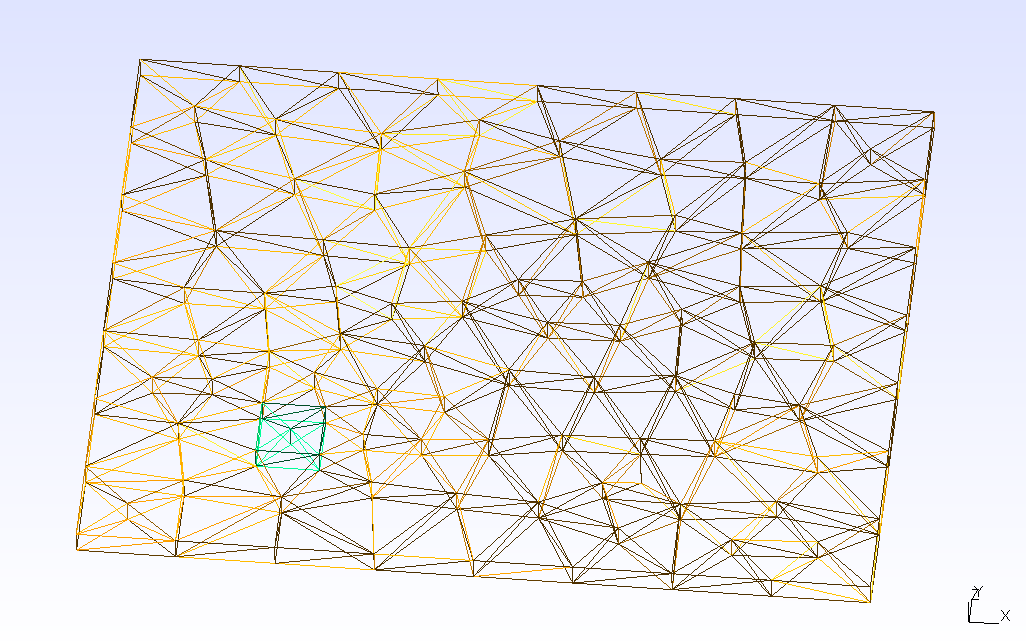
\includegraphics[width=\linewidth]{211Nodes_cavityWithSourceAt650x500y_75_DLI.PNG}
  \caption{211 Node Mesh, No Split}
  \label{fig:mesh39}
\end{figure}

The mesh with 211 Nodes is not very fine, but runs fast. Unfortunately, after just 1 split, it is too much for my PC to handle, but may do better in terms of results. It can be seen from the figure that the cells in green are the refinement area for the source.

The results for 211 Nodes in the Voltage response were measured at the source which was x = 0.0625 meters, y = 0.05 meters. The Voltage monitor was placed at x = 0.0725m, y = 0.06m.
The voltage is off by several magnitudes compared to what is expected for at the source, but this can be explained due to the need for dividing my result by the area, since I am assuming my current source $I_s$ is equivalent to my current density source $J_s$. 

As can be seen, not much voltage transfers from the source to the monitor, which points to a problem in the code since for a Cavity such as this, even at high frequency, the voltage should still be propagated if the E-field is properly being propagated. We expect the Monitor and the source to have about the same order of magntiude.

With that said, however, it is still proof that the FETD code is working in a sense since there is some voltage coupling to the next mesh cell. This means that the time stepping works to an extent and the $[S]$ and $[T]$ Matrices are properly computed.

The problem of low voltage athe monitor most likely also relates to the DC offset at later time. They are most likely both caused by my treatment of the source where I approximated the forcing vector in \ref{eq:forcing}

Another suitable treatment is an infinitely thin wire, which is given in ~\cite{Edelvik}.

\begin{figure}
  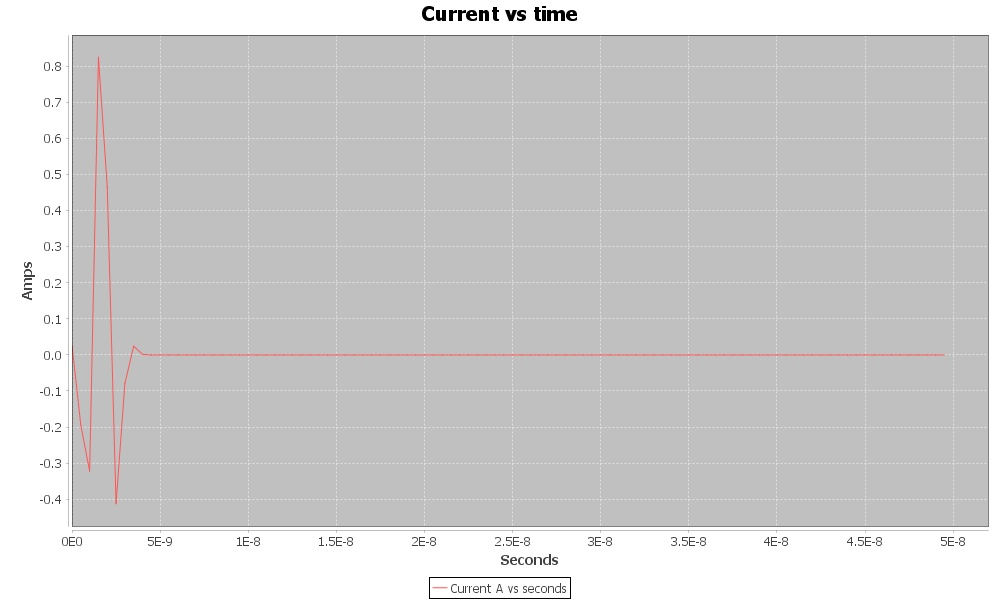
\includegraphics[width=\linewidth]{211Current.jpg}
  \caption{The Current Source input}
  \label{fig:mesh39}
\end{figure}

\begin{figure}
  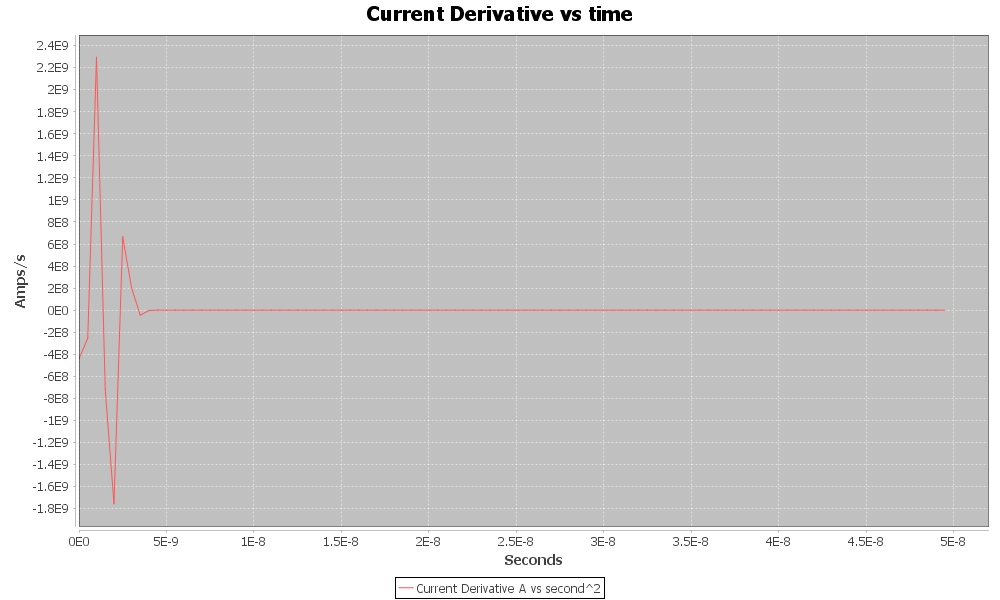
\includegraphics[width=\linewidth]{211CurrentDerivative.jpg}
  \caption{The Current Source input Derivative}
  \label{fig:mesh39}
\end{figure}

\begin{figure}
  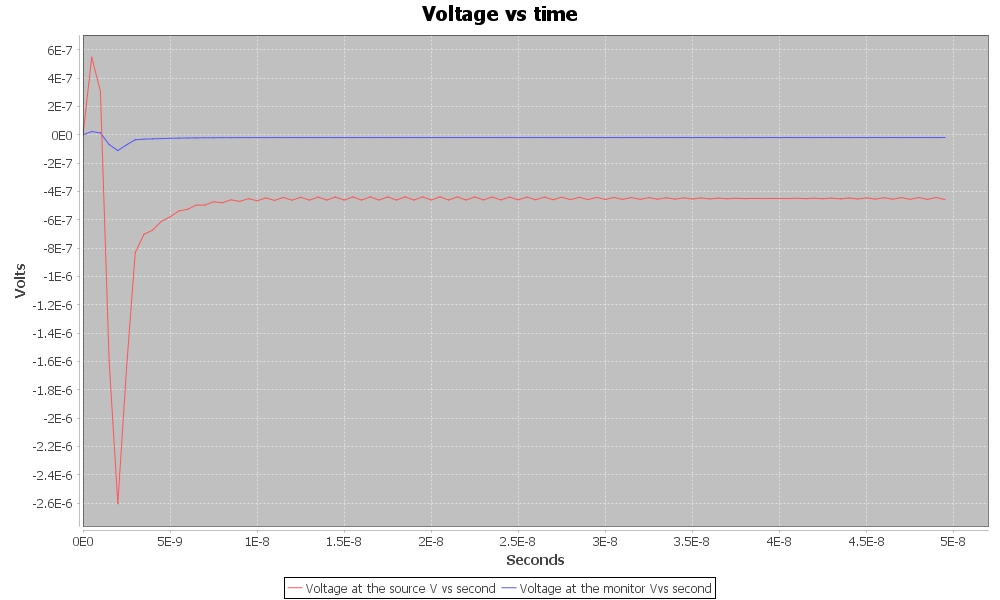
\includegraphics[width=\linewidth]{211Voltages.jpg}
  \caption{The Voltage at the Source in Red. The Voltage at the Monitor in Blue.}
  \label{fig:mesh39}
\end{figure}



\bibliographystyle{unsrt}
\bibliography{FiniteElementAnalysisOfCavitiesBib}

\end{document}

